%!TeX root=../apresentacao.tex
%("dica" para o editor de texto: este arquivo é parte de um documento maior)
% para saber mais: https://tex.stackexchange.com/q/78101/183146

% Apague as duas linhas abaixo (elas servem apenas para gerar um
% aviso no arquivo PDF quando não há nenhum dado a imprimir) e
% insira aqui o conteúdo do seu trabalho. Tome por base o
% arquivo corpo-apresentacao.tex do diretório conteudo-exemplo
% para a definição do título, autoria etc. e estrutura da
% apresentação.

\customtitlepage

% Slide com o qrcode
\showqrcode

\begin{frame}{Overview}
  \overview
\end{frame}

\section{Introduction}

%------------------------------------------------------------------------------
\begin{frame}{Context}
  \begin{itemize}
    \item Programmers use a tool named {\color{red}{compiler}} to generate binaries for their projects
    \begin{itemize}
      \item A {\color{red}{compiler}} is a program that translates code in language $A$ to another language $B$
      \item Remove the needs of coding in assembly
      \begin{itemize}
        \item Cheaper and faster software development
      \end{itemize}
    \end{itemize}
    \item Translation is done serially per file
    \begin{itemize}
      \item Parallel in the number of files
    \end{itemize}
  \end{itemize}
\end{frame}

%------------------------------------------------------------------------------

\begin{frame}{Context}
  \begin{itemize}
    \item Example: compiling a C file
  \end{itemize}
\begin{center}
\tikzstyle{block} = [rectangle, draw, fill=white,
    text width=6em, text centered, rounded corners, node distance=6.5cm, auto, minimum height=2em]
\tikzstyle{line} = [draw, -latex]
\tikzstyle{cloud} = [draw, ellipse,fill=white, node distance=2cm,
    minimum height=2em]
\scalebox{0.6}{
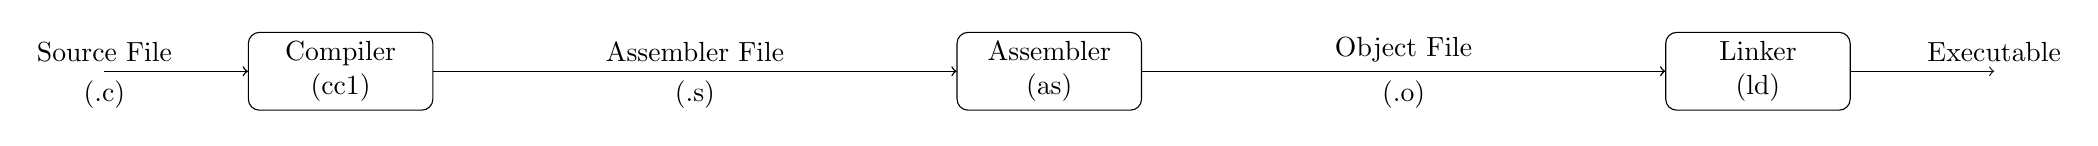
\begin{tikzpicture}[node distance = 3cm, auto]
    % Place nodes
    \node [block]                      (cc1) {Compiler \\ (cc1)};
    \node [block, right of = cc1]      (as) {Assembler\\(as)};
    \node [block, right of = as]       (ld) {Linker\\(ld)};
    \coordinate [left of=cc1]          (fonte);
    \coordinate [right of=ld]    (bin);

    % Draw edges
    \draw[->]    (cc1.east)    -- (as.west)       node[midway, above] {Assembler File};
    \draw[->]    (cc1.east)    -- (as.west)       node[midway, below] {(.s)};
    \draw[->]    (as.east)     -- (ld.west)       node[midway, above] {Object File};
    \draw[->]    (as.east)     -- (ld.west)       node[midway, below] {(.o)};
    \draw[->]    (fonte.west)  -- (cc1.west)      node[pos=0, above] {Source File};
    \draw[->]    (fonte.west)  -- (cc1.west)      node[pos=0, below] {(.c)};
    \draw[->]    (ld.east)     -- (bin.west)      node[pos=1, above] {Executable};
\end{tikzpicture}
}
\end{center}
\end{frame}

%------------------------------------------------------------------------------

\begin{frame}{Context}
  \begin{itemize}
    \item When combined with Makefiles, compilation works like this:
  \end{itemize}

\begin{center}
\tikzstyle{block} = [rectangle, draw, fill=white,
    text width=6em, text centered, rounded corners, node distance=1cm and 1.5cm, auto, minimum height=2em]
\tikzstyle{line} = [draw, -latex]
\tikzstyle{cloud} = [draw, ellipse,fill=white, node distance=2cm and 2cm,
    minimum height=2em, minimum width=2em]
\scalebox{0.6}{
\begin{tikzpicture}[node distance = 3cm, auto]
    % Place nodes
    \node [block]                         (make)   {Makefile};
    \coordinate[right=of make]            (c);
    \node [block, right=of make]          (fonte2) {source2.cpp};
    \node [block, above=of fonte2]        (fonte1) {source1.c};
    \node [block, below=of fonte2]        (fonte3) {fonte3.f90};

    \node [block, right=of fonte1]        (gcc)      {gcc};
    \node [block, right=of fonte2]        (g++)      {g++};
    \node [block, right=of fonte3]        (gfortran) {gfortran};

    \node [block, right=of gcc]           (objeto1) {object1.o};
    \node [block, right=of g++]           (objeto2) {object2.o};
    \node [block, right=of gfortran]      (objeto3) {object3.o};

    \node [block, right=of objeto2]       (ld) {ld};

    \node [block, below=of ld]            (bin) {Executable};

    % Draw edges
    \draw[->]    ([yshift=+0.7em] make.east)   -- (fonte1.west);
    \draw[->]    (make.east)                   -- (fonte2.west);
    \draw[->]    ([yshift=-0.7em] make.east)   -- (fonte3.west);

    \draw[->]    (fonte1.east)    -- (gcc.west);
    \draw[->]    (fonte2.east)   -- (g++.west);
    \draw[->]    (fonte3.east)   -- (gfortran.west);

    \draw[->]    (gcc.east)   -- (objeto1.west);
    \draw[->]    (g++.east)   -- (objeto2.west);
    \draw[->]    (gfortran.east)   -- (objeto3.west);

    \draw[->]    (objeto1.east)   -- ([yshift=+0.7em]ld.west);
    \draw[->]    (objeto2.east)   -- (ld.west);
    \draw[->]    (objeto3.east)   -- ([yshift=-0.7em]ld.west);

    \draw[->]    (ld.south)   -- (bin.north);


\end{tikzpicture}
}
\end{center}
\end{frame}

%----------------------------------------------------------------------------

\begin{frame}{Context}
  \begin{itemize}
    \item What happens if some files takes a really long time to compile?
    \begin{itemize}
        \item C++ blob files generated by other programs
        \item Heavy use of templates
    \end{itemize}
    \item Bottleneck in compilation!
  \end{itemize}
\end{frame}

%------------------------------------------------------------------------------

\begin{frame}{Context}
  \begin{itemize}
    \item Example: GCC compilation (64-threads Opteron machine):
  \end{itemize}

\begin{center}
\includegraphics[width=0.8\paperwidth]{seq-crop.pdf}
\end{center}
\end{frame}

%------------------------------------------------------------------------------

\begin{frame}{Context}
  \begin{itemize}
    \item Example: GCC compilation (64-threads Opteron machine):
  \end{itemize}

\begin{center}
\includegraphics[width=0.8\paperwidth]{power-seq-crop.pdf}
\end{center}
\end{frame}

%------------------------------------------------------------------------------

\begin{frame}{Context}
  \begin{itemize}
    \item In the previous figure:
    \begin{itemize}
        \item Compilation is slow due to suboptimal use of CPU cores
    \end{itemize}
    \item Compilation consumes $19.659Wh$ of power
    \item[]
    \item Can we improve that by parallelizing the compiler?
  \end{itemize}

\end{frame}

%------------------------------------------------------------------------------

\begin{frame}{Context}
  \begin{itemize}
    \item Research Questions:
    \begin{itemize}
        \item \textbf{RQ1} - What is the main point in a compiler that can be improved with parallelism?
        \item \textbf{RQ2} - What is the performance improvement after parallelizing a compiler?
        \item \textbf{RQ3} - When compiling in parallel is faster than compiling sequentially?
        \item \textbf{RQ4} - How does a parallel compiler impact the power consumption?
    \end{itemize}
  \end{itemize}

\end{frame}

%------------------------------------------------------------------------------
\section{Theoretical Background}
%------------------------------------------------------------------------------
%------------------------------------------------------------------------------
\begin{frame}{Theorectical Background}
  \begin{block}{Problems}
    \begin{itemize}
      \item Not every part of a compiler can be parallelized
      \begin{itemize}
        \item Parallelizing a industry standard compiler can be challenging
        \item Using only the code for ideas is not viable
      \end{itemize}
      \item Therefore, we must rely on compiler theory
      \begin{itemize}
          \item Can provide us strategies to parallelize on a compiler agnostic way
      \end{itemize}
      \item If theory says it is possible, it is a good option to try
    \end{itemize}
  \end{block}
\end{frame}
%------------------------------------------------------------------------------
\subsection{Parser}
\begin{frame}{Parser}
    \begin{itemize}
        \item Computer language programs are written in text files
        \begin{itemize}
            \item Needs to be \textit{parsed} to create an \textit{Abstract Tree} (AST) 
        \end{itemize}
        \item Parsing usually consists of two analyzers:
        \begin{itemize}
            \item Lexical Analyzer: break the input text into \textit{tokens}
            \item Syntactic Analyzer: read input tokens and try to reduce (or predict)
            to grammar rule
        \end{itemize}
    \end{itemize}
\end{frame}
%------------------------------------------------------------------------------
\subsection{Parser}
\begin{frame}{Parser}
\tikzstyle{block} = [rectangle, draw, fill=white,
    text width=6em, text centered, rounded corners, node distance=9cm, auto, minimum height=2em]
\tikzstyle{line} = [draw, -latex]
\tikzstyle{cloud} = [draw, ellipse,fill=white, node distance=2cm,
    minimum height=2em]

%TODO: Adcionar a tabela de símbolos aqui.
\begin{center}
\scalebox{0.7}{
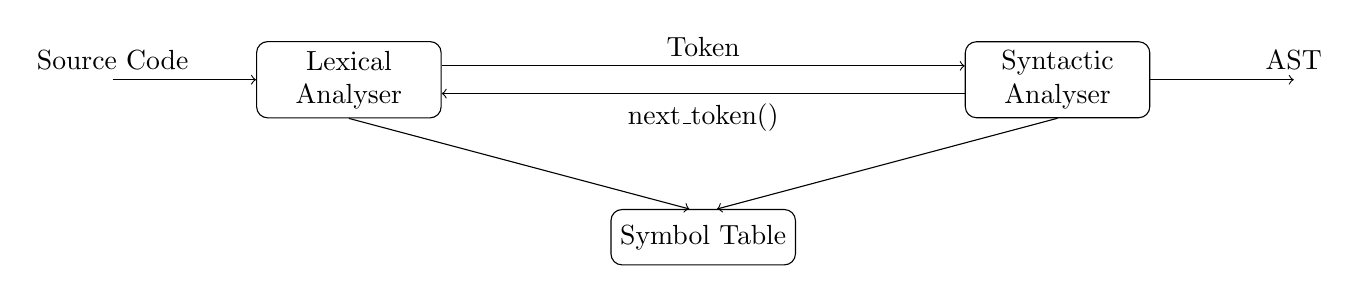
\begin{tikzpicture}[node distance = 3cm, auto]
    % Place nodes
    \node [block]                    (lexico) {Lexical Analyser};
    \node [block, right of = lexico] (sintatico) {Syntactic Analyser};
    \node [block] at (4.5, -2) (symtab) {Symbol Table};
    \coordinate [left of=lexico]     (fonte);
    \coordinate [right of=sintatico] (ast);

    % Draw edges
    \draw[->]    ([yshift=0.5em] lexico.east)       -- ([yshift=0.5em] sintatico.west) node[midway] {Token};
    \draw[->]    ([yshift=-0.5em] sintatico.west)   -- ([yshift=-0.5em] lexico.east)    node[midway] {next\_token()};
    \draw[->]    (fonte.west)                       -- (lexico.west)    node[pos=0, above] {Source Code};
    \draw[->]    (sintatico.east)                   -- (ast.west)   node[pos=1, above] {AST};
	\draw[->]    (sintatico.south)                  -- ([xshift=0.5em]symtab.north);
	\draw[->]    (lexico.south)                     -- ([xshift=-0.5em]symtab.north);

\end{tikzpicture}
}
\end{center}
\end{frame}

%------------------------------------------------------------------------------

\begin{frame}{Parser}
\begin{itemize}
    \item There are two general rules when parsing the input:
    \begin{itemize}
        \item Top-down Parsing: predict the input string from the starting rule $S$
        \item Bottom-up Parsing: reach the starting rule $S$ from the input string
    \end{itemize}
\end{itemize}
\end{frame}

%------------------------------------------------------------------------------

\begin{frame}{Parser}
\begin{itemize}
    \item With the following example grammar:
\begin{center}
\begin{align}
S &\rightarrow E \nonumber \\
E &\rightarrow T + E \; | \; T  \nonumber \\
T &\rightarrow a \times T \; | \; a \nonumber
\end{align}
\end{center}
    \item Input string: $a + a \times a$
    \item Top down parser:
    \begin{itemize}
        \item $ S \Rightarrow E \Rightarrow T + E \Rightarrow a + E \Rightarrow a + T \Rightarrow a + a \times T \Rightarrow a+ a \times a$
    \end{itemize}

\end{itemize}
\end{frame}

%------------------------------------------------------------------------------

\begin{frame}{Parser}
\begin{itemize}
    \item With the following example grammar:
\begin{center}
\begin{align}
S &\rightarrow E \nonumber \\
E &\rightarrow T + E \; | \; T  \nonumber \\
T &\rightarrow a \times T \; | \; a \nonumber
\end{align}
\end{center}
    \item Input string: $a + a \times a$
    \item Bottom up parser (bullet $\bullet$ denotes stack):
    \begin{itemize}
        \item $a + a \times a \Leftarrow T \bullet + a \times a \Leftarrow T + a \times a \bullet \Leftarrow T + a \times T \bullet \Leftarrow T + E \bullet \Leftarrow E \bullet \Leftarrow S \bullet$
    \end{itemize}
\end{itemize}
\end{frame}

%------------------------------------------------------------------------------

\begin{frame}{Parser}
\begin{itemize}
    \item After parsing is complete, an AST is generated
    \item This tree can be used for several analysis:
    \begin{itemize}
        \item Check for semantic errors in the code
        \item Find and Replace optimizations
        \item Calculating size of record type
        \item ... and so on
    \end{itemize}
\end{itemize}
\end{frame}

%------------------------------------------------------------------------------

\begin{frame}{Parser}
\begin{itemize}
    \item AST for the previous example:

\Tree[.S [.E [.T [\textit{a} ]][.E [$+$ ][.T [\textit{a} ][$\times$ ][.T [\textit{a} ]]]]]]

\end{itemize}
\end{frame}

%------------------------------------------------------------------------------
\subsection{Intraprocedural Optimizations}
%------------------------------------------------------------------------------
%------------------------------------------------------------------------------
\begin{frame}{Three-Address Form (3AC)}
\begin{itemize}
    \item Expressions can become arbitrarly large \vspace*{-0.5cm}
    \begin{itemize}
        \item[] $$y = x \times x + x \times x$$ \vspace*{-0.3cm}
        \item Hard to simplify expressions
    \end{itemize}
    \item Idea: break expressions so that it have a maximum of two operands
    and one assignment \vspace*{-0.3cm}
    \begin{align}
          t_1 &= x \times x \nonumber \\
          t_2 &= x \times x \nonumber \\
            y &= t_1 + t_2 \nonumber
    \end{align} \vspace*{-0.6cm}
    \item Clearly, $t_1 = t_2$, so expression is $2x^2$
    \item Also useful on register allocation step
\end{itemize}

\end{frame}

\begin{frame}[plain]
  \includegraphics[width=\textwidth]{interscity-logo}
\end{frame}

\begin{frame}[standout]
  This is a problem!
\end{frame}

\begin{frame}{Goals}
  \begin{block}{Functional requirements}
    \begin{itemize}
      \item Integration and Management of \alert{IoT} Devices
      \item Data Acquisition, Storing, and Processing
      \item Context-awareness
      \item City Resource Discovery
      \item Geolocation-based Services
      \item External data access
    \end{itemize}
  \end{block}
\end{frame}

\section{Concepts}

\begin{frame}{Concepts}
  \begin{columns}[t]
    \col
      \begin{coloredblock}{red!90!black}{Functional requirements}
        \begin{itemize}
          \item Integration and Management of IoT Devices
          \item Data Acquisition, Storing, and Processing
          \item Context-awareness
          \item City Resource Discovery
          \item Geolocation-based Services
          \item External data access
        \end{itemize}
      \end{coloredblock}

    \col
      \begin{coloredblock}{red!90!black}{Non-functional requirements}
        \begin{itemize}
          \item Interoperability
          \item Scalability
          \item Security
          \item Privacy
          \item Evolvability
          \item Adaptability
        \end{itemize}
      \end{coloredblock}
  \end{columns}
\end{frame}

\begin{frame}{Theorems and proofs}
  \pause
  \begin{theorem}[An example theorem]
    Theorem\dots
  \end{theorem}

  \pause
  \begin{example}[An example of an example]
    Example\dots
  \end{example}

  \pause
  \begin{proof}[An example proof]
    Proof\dots
  \end{proof}

  \pause
  \begin{definition}[An example definition]
    Definition\dots
  \end{definition}

  \pause
  \begin{proposition}[An example proposition]
    Proposition\dots
  \end{proposition}
\end{frame}

\section{Related Works}

\begin{frame}{Related Works}
\end{frame}

\section{Methodology}

\begin{frame}{Methodology}
\end{frame}

\section{Results}

\subsection{Validation and Analysis}

\begin{frame}{Validation}
\end{frame}

\begin{frame}{Case Study}
\end{frame}

\section{Conclusion and Future works}

\begin{frame}{Conclusion and Future works}
\end{frame}

\section{References}

\begin{frame}[allowframebreaks]{References}
  \nocite{bronevetsky02, schmidt03:MSc, FSF:GNU-GPL, CORBA:spec, MenaChalco08, natbib, biblatex, eco:09}
  \printbibliography
\end{frame}

% Recapitulando
\begin{frame}{\insertshorttitle}
  \overview

  % \begin{center} acrescenta espaço vertical;
  % como possivelmente temos bem pouco espaço aqui,
  % vamos usar centering
  {%
    \centering\noindent%
    \url{https://gitlab.com/link-of-your-repository}\par
  }

\end{frame}

\showqrcode

\appendix

\begin{frame}{Extra info}
  \begin{itemize}
    \item It is often useful to have some extra slides addressing likely questions from the audience at the end of the presentation
    \item By putting them after the ``appendix'' command, they are not counted in the page count indicator
  \end{itemize}
\end{frame}



\input{extras/aviso-conteudo}
\avisoApresentacao
